\clearpage

\section{IP Tunnel}

\begin{tcolorbox}	
	\begin{tabular}{p{2.75cm} p{0.2cm} p{10.5cm}} 	
		\textbf{Header File}   &:& ip$\_$tunnel$\_*$.h \\
		\textbf{Source File}   &:& ip$\_$tunnel$\_*$.cpp \\
        \textbf{Version}       &:& 20180815 (Jo\~ao Coelho) \\
	\end{tabular}
\end{tcolorbox}

This block accepts one input signal and transmits it. The same block, on the other machine, accepts the signal and outputs it. It takes samples out of the buffer until the buffer is empty.

\subsection*{Input Parameters}

\begin{table}[h]
	\centering
	\begin{tabular}{|c|c|p{30mm}|c|ccp{60mm}}
		\cline{1-4}
		\textbf{Parameter} & \textbf{Type} & \textbf{Values} &   \textbf{Default}& \\ \cline{1-4}
		numberOfSamples & long int & any & $-1$ \\ \cline{1-4}
        displayNumberOfSamples & bool & true/false & true \\ \cline{1-4}
		numberOfTrials & int & any & $5$ \\ \cline{1-4}
		numberOfRepetions & int & any & $3$ \\ \cline{1-4}
		ipAddressServer & string & any & "127.0.0.1" \\ \cline{1-4}
		tcpPort & int & any & $54000$ \\ \cline{1-4}
	\end{tabular}
	\caption{IP Tunnel input parameters}
	\label{table:ipt_in_par}
\end{table}

\subsection*{State Variables}

\begin{table}[h]
	\centering
	\begin{tabular}{|c|c|p{30mm}|c|ccp{60mm}}
		\cline{1-4}
		\textbf{Parameter} & \textbf{Type} & \textbf{Values} &   \textbf{Default}& \\ \cline{1-4}
		alive & bool & true/false & true \\ \cline{1-4}
        finished & bool & true/false & false \\ \cline{1-4}
	
	\end{tabular}
	\caption{IP Tunnel state variables}
	\label{table:iptunnel_st_var}
\end{table}

\subsection*{Methods}
%
IPTunnel(vector$<$Signal *$>$ \&InputSig, vector$<$Signal *$>$ \&OutputSig)
\bigbreak
void initialize(void);
\bigbreak
bool runBlock(void);
\bigbreak
void ipTunnelSendInt(int space);
\bigbreak
int ipTunnelRecvInt();
\bigbreak
int ipTunnelPut(T object);
\bigbreak
bool server();
\bigbreak
bool client();


\subsection*{Functional Description}

The IP Tunnel block transmits all elements contained in the signal passed as input. This block is duplicated onto two machines, one with input and other with output signals. After being executed the input signal's buffer will be empty and will transmit this signal to the output of the other block. It uses an architecture Server - Client, to establish a TCP/IP channel between the two blocks. The block without input signals is the server (receiver) and the block with input signals is the client (transmitter). After the connection is established, the server sends the space of its buffer (maximum of signal size that can be received) and client responds with process (the size of the signal that is going to be transmitted) and with an integer representing the type of the signal. Subsequently, the transmission of the signal starts.

\begin{figure}[h]
	\centering
	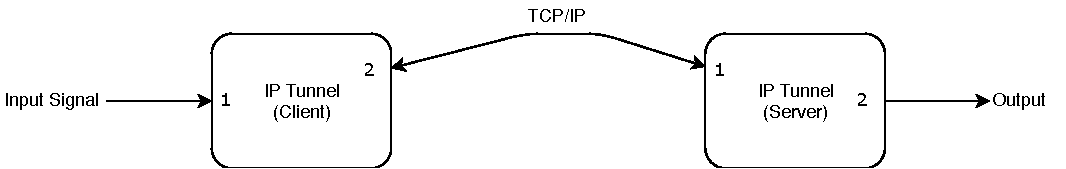
\includegraphics[width=0.6\textwidth, height=5cm]{./lib/ip_tunnel/figures/StructureTCPIP.pdf}
	\label{IP Tunnel Block}\caption{IQ Modulator block}
\end{figure}